\documentclass[journal]{IEEEtran}
\usepackage{graphicx} % Required for inserting images
\usepackage{array}
\usepackage{booktabs}
\usepackage{amsmath}
\usepackage{float}
\usepackage{url}
\title{Visual Speech Recognition in Tai Phake}
\author{abc, efg, hij, klmnop}
\date{October 2026}
\raggedbottom
\begin{document}
\maketitle
\begin{abstract}
    Visual Speech Recognition is used to identify spoken words using only mouth movements. Although a lot of work is done in high resource languages, developing a VSR system for low resource languages remains challenging because of scarce digital resources and datasets. This paper explored VSR for Tai Phake, an endangered language of Assam with approximately 2,000 people speaking the language in the whole world. We compared three deep learning architectures—EfficientNetB0 combined with a Bidirectional LSTM (BiLSTM), EfficientNetB0 combined with Bidirectional GRU (BiGRU), and EfficientNetB0 combined with a lightweight Transformer encoder. Using a speaker-independent 5-fold GroupKFold cross-validation framework on a custom digit dataset, the EfficientNetB0–BiLSTM model achieves a target accuracy of 90.4\%, surpassing the BiGRU (87.2\%) and Transformer (86.8\%) variations. Analyzing the errors, the majority of the errors are due to similar visual mouth movements and phonemic similarities. This shows how important it is to check the data and make sure the sound and the look match, for speech technologies that have little data.

    \textbf{Keywords}: Visual Speech Recognition, Low Resource Language, Tai Phake, EfficientNetB0, Bidirectional Long Short Term (BiLSTM), Bidirectional Gated Recurrent Unit(BiGRU), Transformer, Digit Recognition
\end{abstract}


\section{Introduction}

Visual Speech Recognition (VSR), also called lip-reading, is the process of recognizing speech by observing the movements of a person's lips and mouth in a video. The computer studies the changes in mouth shape over a sequence of video frames and uses them to predict the words spoken by a person. This makes it possible to study speech without using audio as input. Visual speech recognition can be useful when audio is not available or when speech cannot be heard clearly \cite{fernandezlopez2018survey}.

With the development of deep learning, researchers have developed different models that can learn useful patterns from video frames and study how the mouth changes over time. The availability of large video datasets has also helped researchers train and compare different advanced models. For example, \cite{chung2016lipreading} introduced the Lip Reading in the Wild (LRW) dataset for recognizing 500 English word classes from videos collected from BBC television programs. Later, \cite{chung2017sentences} introduced the Lip Reading Sentences in the Wild dataset, which focused on recognizing complete phrases and sentences instead of only a fixed set of words. However, developing similar systems for languages with limited data remains a challenge.

One major problem in visual speech recognition is the need for a sufficient number of labelled video samples. A model must learn the mouth movements associated with different words from many examples. The samples should also include differences between speakers, such as their speaking style, mouth shape, and speed of speech. When only a small amount of data is available, it becomes difficult to train a model that works well for people who were not included in the training data. Research on low-resource languages has also identified the lack of digital data and other language resources as an important problem in developing language technologies \cite{magueresse2020low}. Therefore, building language-specific datasets is an important step towards studying visual speech recognition for languages that have received less attention.

India is a multilingual country where people speak many different languages. The Census of India 2011 language report lists 22 Scheduled Languages and 99 Non-Scheduled Languages \cite{census2011language}. Researchers have started exploring visual speech recognition for several Indian languages. For Hindi, \cite{patil2019hindi} developed a lip-reading approach using mouth-related features and a Long Short-Term Memory (LSTM) network. \cite{rudregowda2023kannada} studied visual speech recognition for Kannada using a VGG16-based convolutional neural network. \cite{kulkarni2024marathi} developed a Marathi lip-reading dataset and examined different neural network approaches. These studies show that language-specific video data and suitable models are important parts of building lip-reading systems for Indian languages.

Assam is a state in Northeast India with many linguistic and cultural communities. Assamese is widely used in the state, while Bodo, Mising, Tai, and other languages are also part of its linguistic diversity. Some research has also been carried out on these languages. \cite{prasad2025analysis} studied Assamese digit recognition using deep learning and developed a custom video dataset for their work. Their study used a CNN-LSTM model to learn features from lip movements. More recently, \cite{lyngdoh2026khasi} studied lip-reading for Khasi digits from zero to nine. They collected videos from nine speakers and used MediaPipe to extract lip-related features before applying machine learning classifiers. These studies provide useful examples of how visual speech recognition can be studied using data collected for a particular language. However, the tasks and methods used in these studies are different, and further research is still needed for many other languages spoken by smaller communities.

A lot of the history of Assam is connected with the Tai-speaking communities. The Tai-Ahoms migrated to present-day Assam in the thirteenth century under the leadership of Siu-kha-pha, who ruled for about 600 years, from the thirteenth to the nineteenth century. The people belonging to the Tai Phake community migrated in and around 1775 from the Hu-Kwang Valley to Assam in search of a better life\cite{lahkar2019origin}. Tai Phake, also called Phakial, is a Tai-speaking language used by a small community in Upper Assam. The Scheme for Protection and Preservation of Endangered Languages reports a population estimate of around 2,000 Tai Phake speakers\cite{deka2025studying}. This makes Tai Phake an endangered language of India. The people of this community mainly live in the Dibrugarh and Tinsukia districts of Assam \cite{sppeletaiphake}. \cite{morey2005tailanguages} documented Tai Phake and other Tai languages of Assam, including their grammar, sound system, vocabulary, and writing system. Such studies provide useful information about the language and its use within the community.

Tai Phake also has linguistic features that make it an important subject for further study. \cite{morey2020syllable} describes six lexical tones in Tai Phake, along with vowel sounds and differences in vowel length. These features are important parts of the language. However, a visual-only recognition system does not receive all the information available in spoken audio. It must learn from the visible movements of the lips and mouth. Some differences between spoken forms may not be clearly visible in a video. Therefore, it is important to examine how well visual speech recognition can distinguish the selected Tai Phake digit classes using mouth movements alone.

Although previous studies have examined Tai Phake from linguistic and cultural perspectives, our literature search could not identify a published visual speech recognition system or a dedicated VSR dataset specifically for Tai Phake. This points to a gap in the use of video-based methods for recognizing Tai Phake speech. Developing a VSR dataset for this language can provide a starting point for studying this problem. It can also help researchers understand which parts of the recognition process work well and which parts need further improvement.

Collecting a dataset for a low-resource language can be difficult. Researchers need access to speakers, suitable recording conditions and enough examples for each target class. The videos must be checked and labelled carefully so that the training samples match the correct words. Differences between speakers must also be considered. If videos from the same speaker are used in both training and validation, the evaluation may not show how well the system works for a new speaker. Hence, the separation of speakers between training and validation is important when evaluating a visual speech recognition model.

To address this research gap, this study develops a visual-only digit recognition system for Tai Phake. A dataset was collected from 30 speakers, with recordings covering 11 target classes labelled from d0 to d10. The video frames are processed to extract the lip regions using Dlib facial landmarks. The cropped regions are prepared as 96 x 96 pixel images for model training. The study examines three deep learning architectures - EfficientNetB0 with BiLSTM, EfficientNetB0 with BiGRU and EfficientNetB0 with a lightweight Transformer model. These models are evaluated using visual information from the videos, without audio features.

The dataset is divided by speaker, with 24 speakers assigned to training and six different speakers assigned to validation. Augmented versions of a speaker's data remain within that speaker's original partition. This prevents the same base speaker from appearing in both training and validation. The study aims to establish an initial experimental basis for Tai Phake digit recognition, compare the selected models, and identify the challenges that affect recognition performance. The dataset and experiments can provide a starting point for future work on visual speech recognition for Tai Phake and other low-resource languages of Northeast India. We will discuss in Section \ref{sec2}.

\section{Related Work} \label{sec2}

Visual Speech Recognition (VSR) has been studied by researchers using different datasets and deep learning models. Most early progress in this field was made using English because a large amount of video data was available for training and testing. More recent studies have also focused on languages with limited data. In this section, we discuss previous research related to visual speech recognition. The related work is divided into two main categories: international research and national research. The international studies include work on English and other languages, while the national studies focus on languages used in India, including Assamese and Khasi.

\subsection{\textit{International Research}}

One of the important works in visual speech recognition was carried out by Chung and Zisserman in \cite{chung2016lipreading}. They introduced the Lip Reading in the Wild (LRW) dataset, which contains video samples for 500 English word classes collected from BBC television programmes. The dataset includes recordings of different speakers and provides a way to train and test models for word recognition. Later, \cite{chung2017sentences} introduced the Lip Reading Sentences in the Wild (LRS) dataset. Unlike LRW, which focuses on individual words, LRS was developed for recognizing phrases and sentences from videos. Their work also presented a deep learning model that learns to recognize speech from sequences of mouth movements. These datasets became useful resources for testing and comparing visual speech recognition methods.

\cite{ma2022multilingualvsr} studied visual speech recognition across multiple languages. Their work showed that both the model design and the amount of training data affect recognition performance. They explored improvements through data augmentation, model training methods and additional learning tasks. Their study also showed that training data from other languages can help improve visual speech recognition. This is important for low-resource languages because collecting a large number of video samples for every language is difficult.

Despite this progress, visual speech recognition remains challenging for languages that do not have large video-text datasets. \cite{kim2023lowresource} proposed a method for low-resource lip-reading by combining general speech knowledge learned from a high-resource language with information specific to the target language. The main idea was to reuse useful knowledge from one language instead of training every part of the system from the beginning. Their study examined the method across English, Spanish, French, Italian and Portuguese. Although their approach also used language-specific audio information, the work is relevant because it addresses the difficulty of training lip-reading systems when video data are limited.

Researchers have also worked on creating datasets for languages that have received less attention. \cite{rahmatullah2024idlr} released the Indonesian Lip Reading (ID-LR) dataset in 2024. It contains 105,300 videos covering 230 Indonesian word classes. The dataset provides separate training, validation and testing sets, making it useful for further work on Indonesian lip-reading. Another example is the LipBengal dataset, introduced in \cite{lipbengal2025}. This dataset contains visual data from 150 speakers and covers 54 Bengali classes, including phonemes, alphabets and symbols. The recordings were collected under different conditions to provide data for future lip-reading research. These datasets show the value of preparing language-specific visual data before developing and comparing recognition models.

\cite{peymanfard2024armanav} introduced the Arman-AV dataset for Persian. It contains about 220 hours of video recordings from 1,760 speakers and was designed to support lip-reading as well as other speech-related tasks. The authors also studied visemes, which are groups of speech sounds that can produce similar visible mouth movements. Their work is useful for understanding the role of dataset size, speaker variation and visible mouth patterns in lip-reading. However, Arman-AV is an audio-visual dataset, whereas the system developed in the present study uses video and lip movements only.

These international studies show that large datasets have helped improve visual speech recognition in several languages. They also show that the lack of video data remains a problem for languages with fewer digital resources. Therefore, collecting suitable video samples and testing models on speakers who were not used during training are important parts of research in this area.

\subsection{\textit{National Research}}

In India, researchers have explored visual speech recognition for languages such as Hindi, Kannada, Marathi, Indian English, Assamese and Khasi. However, the datasets and methods used in these studies differ, depending on the language and the task being recognized.

\cite{patil2019hindi} developed an LSTM-based lip-reading system for Hindi using the Devanagari script. They collected video recordings from 50 people and used lip-related geometric features to recognize words and sentences. Their study reported different accuracy levels for tasks involving different numbers of words. This work showed that a language-specific dataset could be created when a suitable public dataset was not available. It also showed that recognizing complete sentences is more difficult than recognizing a smaller set of words.

\cite{rudregowda2023kannada} studied visual speech recognition for Kannada using a VGG16-based convolutional neural network. Their work used visual features from video sequences to recognize speech in Kannada. In another study, Kulkarni and Kirange \cite{kulkarni2024marathi} developed a Marathi lip-reading dataset and examined different neural network methods. Their work focused on collecting language-specific data and using it to train models for Marathi. These studies show that both dataset preparation and model selection are important when building lip-reading systems for Indian languages.

In \cite{indian2024audiovisual}, also developed a custom dataset for Indian English speech recognition. They used Dlib to extract visual features from the mouth region and an LSTM-based network for visual speech recognition. Their paper examined audio-based, visual-based and combined audio-visual methods. The visual-only part of their study is particularly relevant to the present work because it uses mouth information extracted from video. In our project, however, audio features and audio-visual combination are not used.

More recently, \cite{prasad2025analysis} studied lip-reading of Assamese digits using deep learning. They created a custom dataset of Assamese digit videos and compared different model architectures. Their CNN-LSTM model achieved a reported accuracy of 83\%. This study is closely related to the present work because it focuses on digit recognition using lip movements in a language spoken in Assam. It also provides a useful example of how a dataset can be collected for a regional language and used to train a deep learning model.

In contrast to this, \cite{lyngdoh2026khasi} studied lip-reading for the Khasi language, which is spoken in Northeast India. They collected digit videos from nine speakers covering the classes from zero to nine. They extracted lip-related features using MediaPipe and applied Principal Component Analysis (PCA) before training Support Vector Machine (SVM) and K-Nearest Neighbors (KNN) classifiers. The authors reported test accuracies of 94.44\% for SVM and 80.86\% for KNN. Their study is particularly relevant because it focuses on digit recognition for a language spoken in the same broad region as Tai Phake. However, these results should not be compared directly with results from other studies unless the datasets and evaluation methods are also comparable.

The reviewed Indian studies show that lip-reading research has been carried out for several languages, including Assamese and Khasi. However, the methods, dataset sizes and recognition tasks vary between studies. In our literature search, we did not identify a published visual speech recognition system or a dedicated VSR dataset specifically for Tai Phake. This leaves room for further work on recognizing Tai Phake speech from lip movements alone.

The present study addresses this gap by collecting video recordings of Tai Phake digits and comparing different deep learning models. The dataset contains 11 classes, labelled from d0 to d10, recorded from 30 speakers. The mouth regions are extracted from video frames and prepared for model training. The data are divided by speaker so that the speakers used for validation are not included in the training set. Unlike studies that use audio or combine audio with video, this work focuses only on visual information. The aim is to establish an initial baseline for Tai Phake digit recognition and identify the challenges that need to be addressed in future work.The methodologies will be discussed in section II.

\section{Methodology}
In this work, we have included three models: EfficientNetB0-BiLSTM, EfficientNetB0-BiGRU and EfficientNetB0 Transformer. Then we compared the accuracies we got after training and testing these models. The workflow of the proposed work is given in Fig. \ref{fig:architecture_diagram}.
\begin{figure}[!t]
    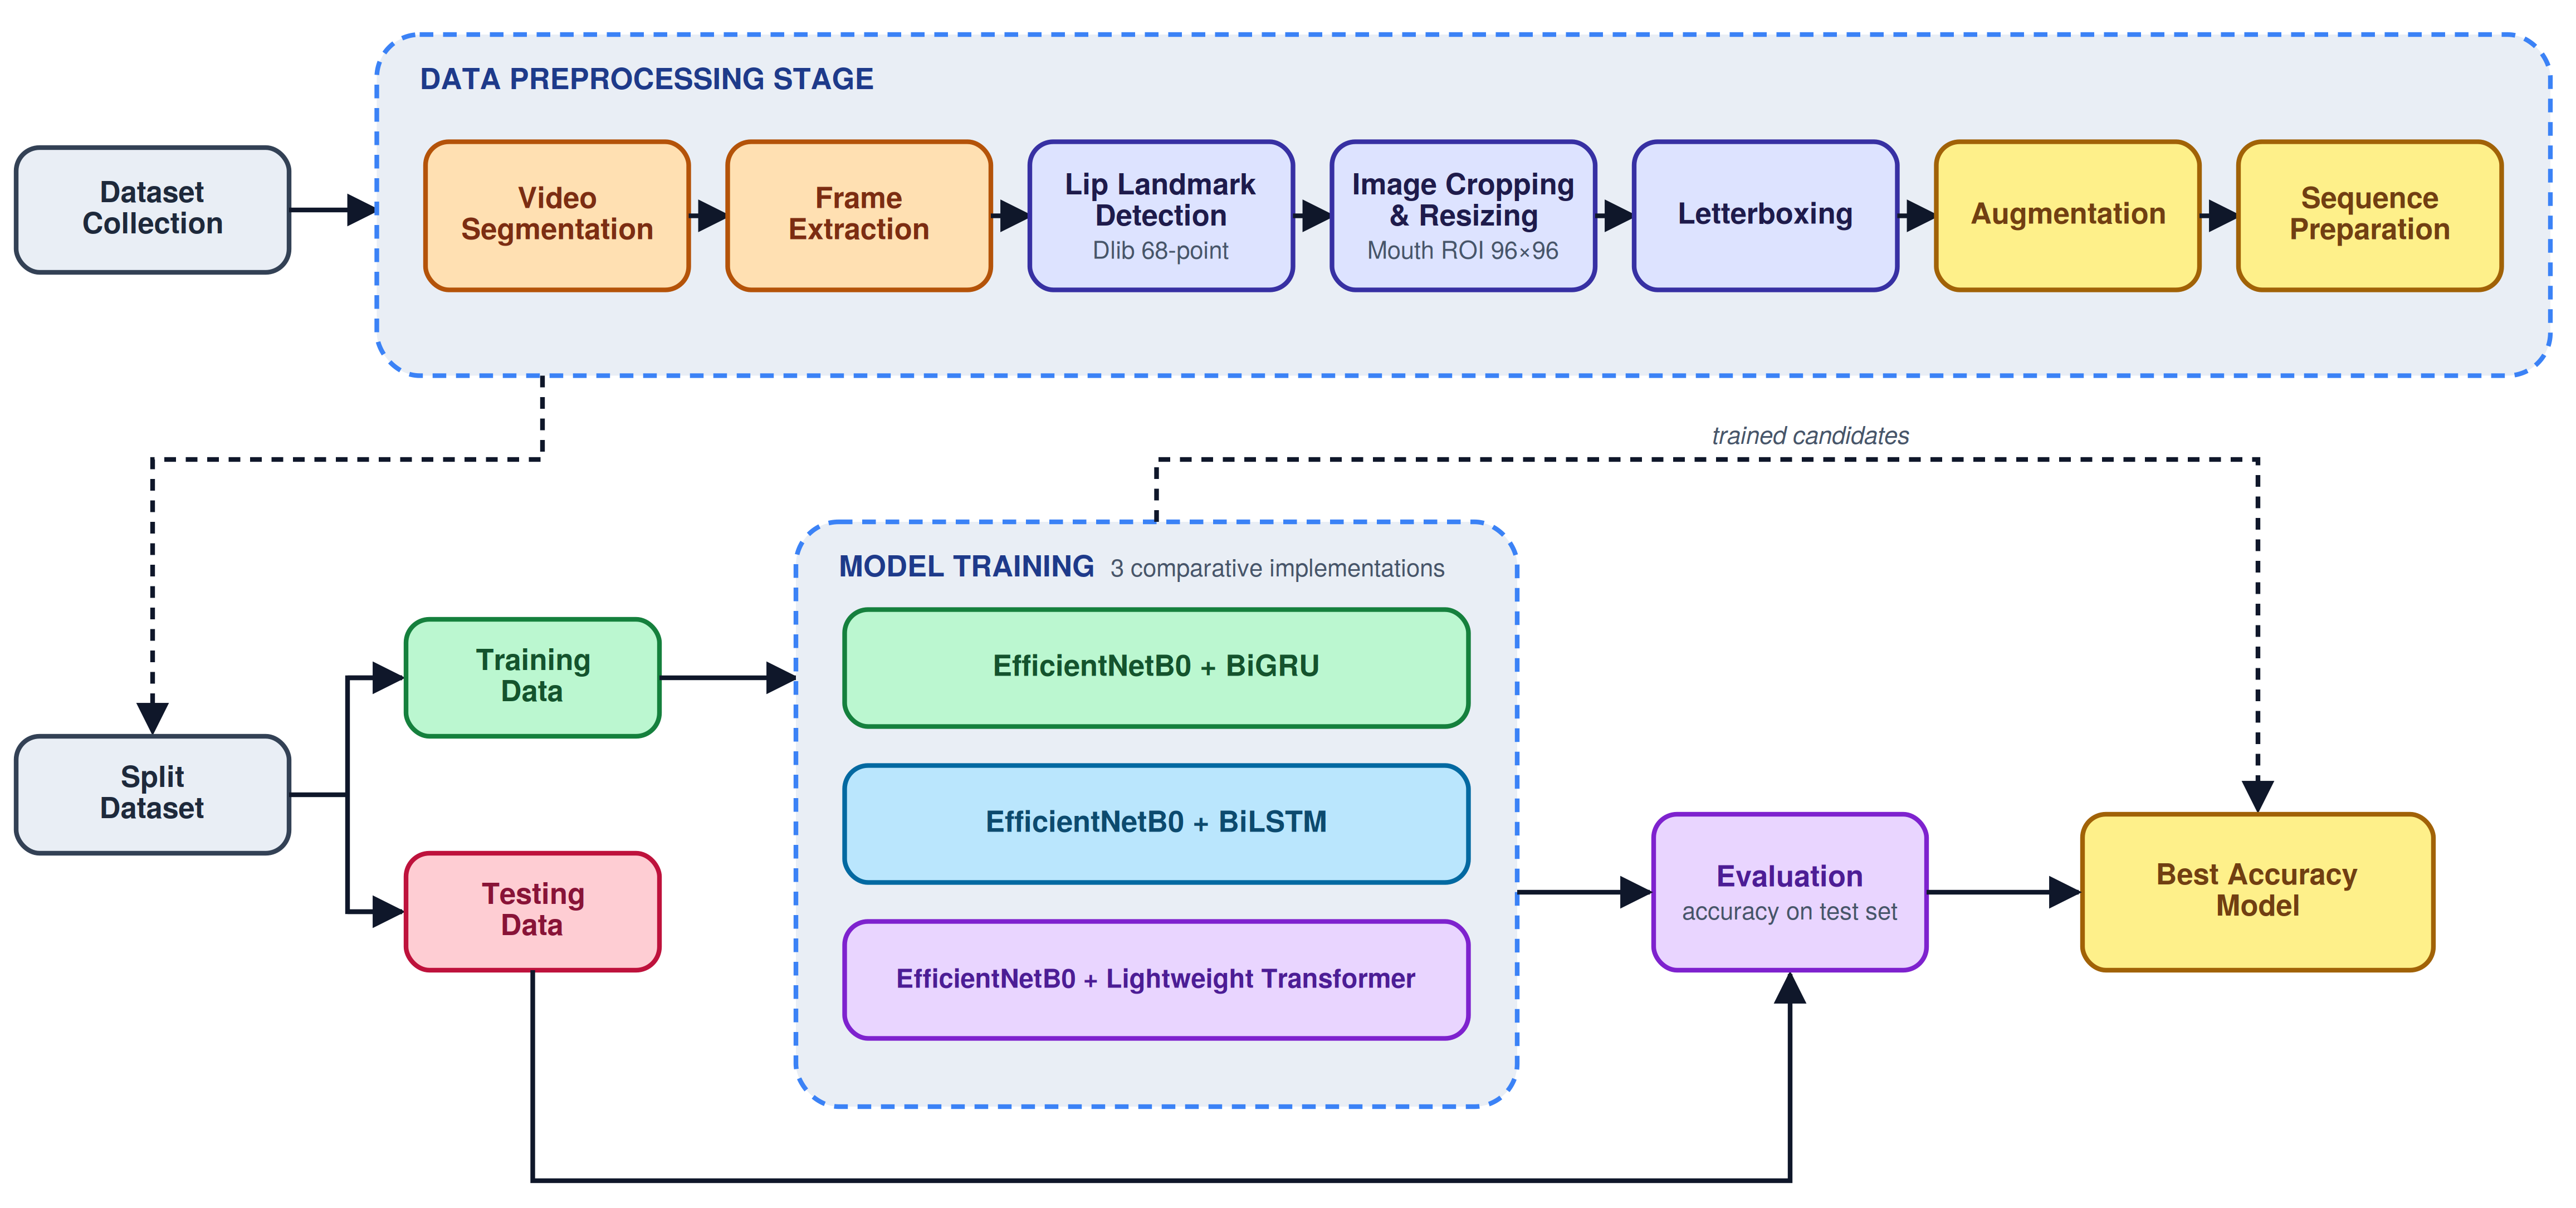
\includegraphics[width=1.0\linewidth]{workflow_restyled (1).png}
    \caption{Architecture diagram}
    \label{fig:architecture_diagram}
\end{figure}

\subsection{Dataset Collection and Preprocessing}
The Tai Phake Visual Speech Recognition dataset contains 330 video samples collected from 30 speakers, including 15 male and 15 female participants. Each speaker recorded digits from 0 (Pao) to 10 (Sip), giving 11 digit classes. The videos were recorded using a phone camera at 30 frames per second (FPS) against a plain, light-colored background. They were stored in MP4 format at a resolution of $720 \times 720$ pixels. Each video contains a single digit. The dataset is organized into speaker folders named `s{speakerNo}`, with video files named `d{clipIndex}.mp4`. This structure helps track speaker identities and digit labels during preprocessing and supports speaker-independent data splitting.

\begin{figure}[htbp]
    \centering
    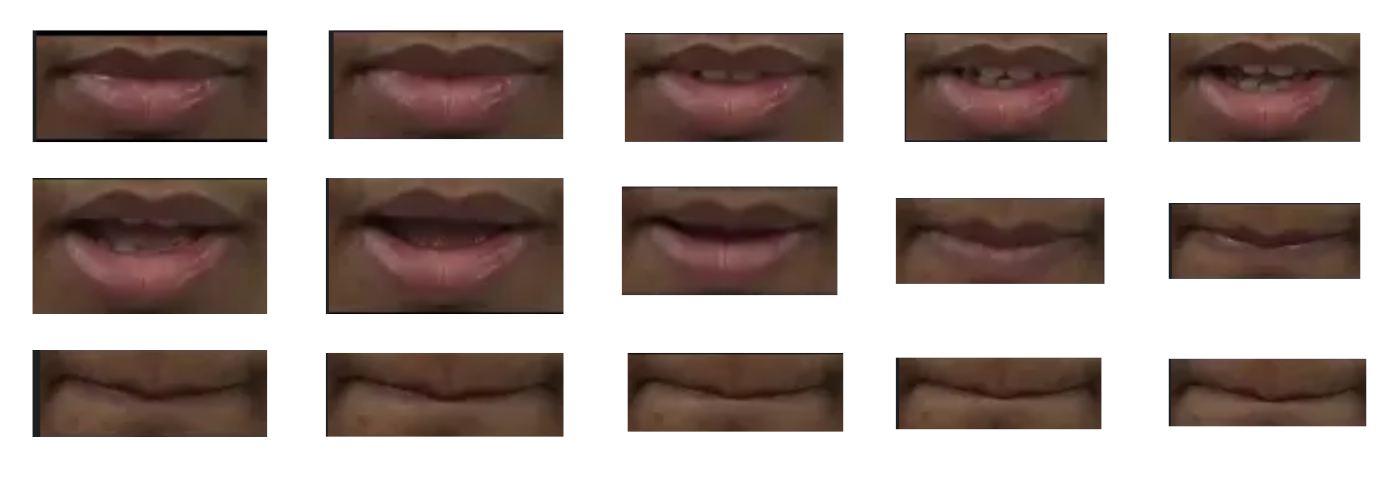
\includegraphics[width=0.9\linewidth]{LIPS_crop.png}
    \caption{Example of detected lips}
    \label{fig:ROI}
\end{figure}
The videos were converted into image sequences for model training and testing. Continuous recordings were manually divided into individual digit clips using Microsoft Clipchamp and Kdenlive. This removed unwanted portions from adjacent recordings. Dlib was used for face detection and facial landmark extraction to identify the mouth region. Similar methods have been used in lip-reading systems \cite{attricnn}. The extracted frames were kept in sequential order to preserve lip movement information.

The extracted mouth images were resized to three tested resolutions: $96 \times 96$, $128 \times 64$, and $112 \times 112$ pixels. After visual evaluation, we selected $96 \times 96$ pixels because it preserved lip features with less distortion and unwanted background content. All frames were standardized to provide consistent model input. The original videos were recorded at 30 FPS, and the extracted image sequences were prepared for further processing and model training.

Data augmentation was applied to increase data diversity and reduce overfitting \cite{shorten2019survey}. Small transformations were used to preserve important lip features and movements. Translation was limited to $\pm3$ pixels, rotation to $\pm3^\circ$, and scaling to 0.97--1.03. Contrast ranged from 0.92--1.08, while brightness ranged from $-10$ to $+10$. Gaussian noise ($\sigma = 1.0$--$3.5$) was applied with a 50\% probability. Gaussian blur used a $3 \times 3$ kernel with $\sigma = 0.5$ and a 30\% probability. Border reflection was used to handle image boundaries, and JPEG quality was set to 95. These small changes increased data variation while preserving the visual information needed for recognition.
After data preprocessing, Section IV presents the proposed models used for Tai Phake visual speech recognition.
\begin{table}[!t]
    \caption{Phakial digits, their transliteration and the number of samples}
    \centering
    \begin{tabular}{c|c|c}

        \textbf{Digit} & \textbf{Transliteration} & \textbf{No. of Samples} \\
        \hline
        0              & Pao                      & 80                      \\
        1              & Naung                    & 80                      \\
        2              & Song                     & 80                      \\
        3              & Saam                     & 80                      \\
        4              & Si                       & 80                      \\
        5              & Haa                      & 80                      \\
        6              & Howk                     & 80                      \\
        7              & Cheit                    & 80                      \\
        8              & Peat                     & 80                      \\
        9              & Kao                      & 80                      \\
        10             & Sip                      & 80                      \\
    \end{tabular}
    \vspace{0.5cm}

    \label{taiphake_digits}
\end{table}

\section{Proposed Models}

\subsection{Shared Preprocessing \& Spatial Backbone}
To ensure a strictly controlled, rigorous comparison, all three proposed architectures share an identical spatial front-end, input preprocessing pipeline, and classification head. Each video clip is standardized to 30 frames at $128 \times 128$ spatial resolution in 3-channel RGB, producing an input shape of $(B, 30, 128, 128, 3)$.

Spatial features are extracted using the EfficientNet-B0 architecture pre-trained on ImageNet \cite{tan2019efficientnet}, with a total backbone parameter count of 5.3 million. All Batch Normalization layers are frozen during training to preserve pre-trained feature statistics under small-batch fine-tuning ($B=16$). Spatial Global Average Pooling (GAP) is applied per frame, transforming each $128 \times 128$ image into a 1,280-dimensional feature embedding, yielding a temporal sequence of 30 feature vectors: $(B, 30, 1280)$.

All models share an identical classifier head: a fully connected linear layer mapping the 256-D pooled temporal representation directly to the 11 target digit classes ($d_0$ to $d_{10}$), followed by Softmax activation ($256 \times 11 + 11 = 2,827$ parameters).

\begin{figure}[h]
    \centering
    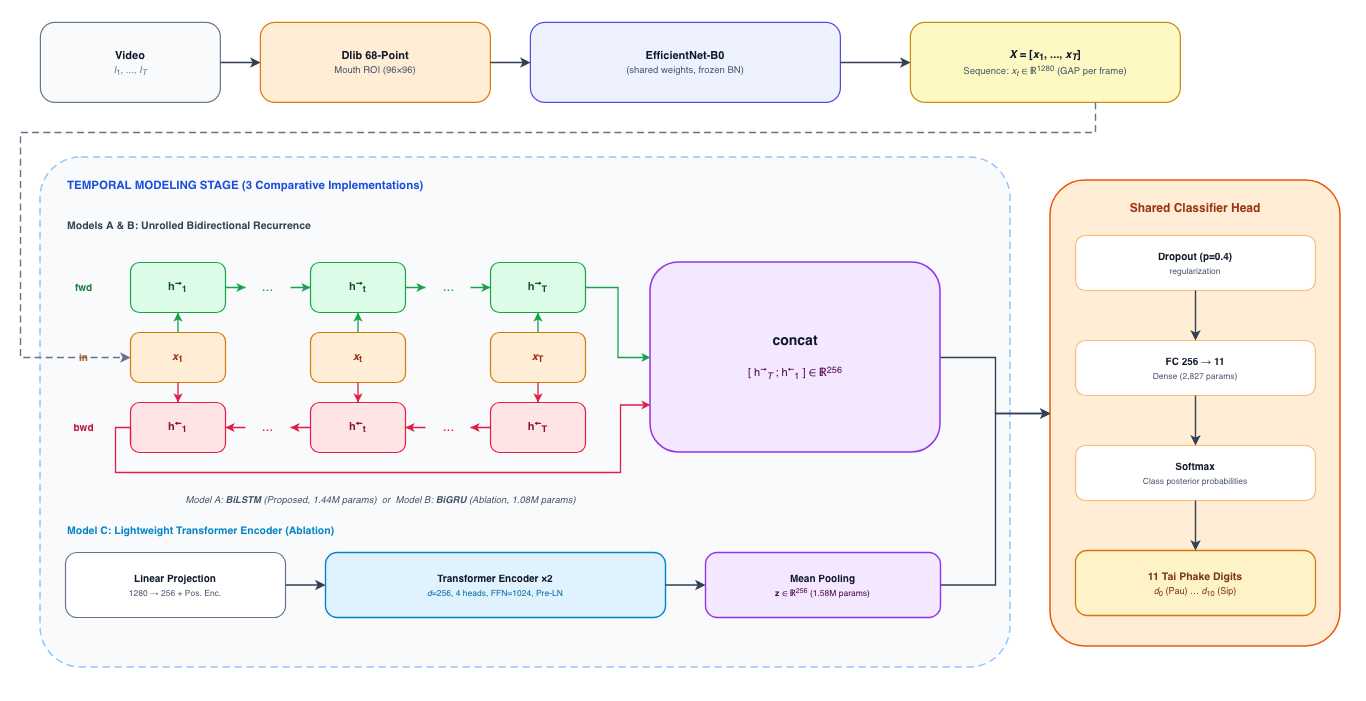
\includegraphics[width=1.0\linewidth]{architecture_combined.drawio.png}
    \caption{Proposed Architecture for Tai Phake Digit Recognition Using Visual Speech Recognition.}
    \label{fig:architecture_combined}
\end{figure}

% Table I: Model comparison with 3 horizontal lines and enhanced row spacing
\begin{table}[!t]
    \centering
    \caption{Model Comparison: Architecture Configurations and Experimental Evaluation Summary}
    \label{tab:proposed_models}
    \fontsize{5.5pt}{7.0pt}\selectfont
    \setlength{\tabcolsep}{1.2pt}
    \renewcommand{\arraystretch}{1.22}

    \begin{tabular}{>{\raggedright\arraybackslash}p{2.30cm}
            >{\raggedright\arraybackslash}p{1.95cm}
            >{\raggedright\arraybackslash}p{1.95cm}
            >{\raggedright\arraybackslash}p{2.20cm}}
        \hline
        \textbf{Parameter}                                                        &
        \textbf{Model A (Proposed)}                                               &
        \textbf{Model B (Ablation)}                                               &
        \textbf{Model C (Ablation)}                                                                                                 \\
        \hline
        \textbf{CNN Backbone} \cite{tan2019efficientnet}                          &
        EfficientNet-B0 (ImageNet)                                                &
        EfficientNet-B0 (ImageNet)                                                &
        EfficientNet-B0 (ImageNet)                                                                                                  \\[1.5pt]
        \textbf{Backbone params}                                                  &
        5.3\,M                                                                    & 5.3\,M          & 5.3\,M                        \\[1.5pt]
        \textbf{Input Shape}                                                      &
        $(B, 30, 128, 128, 3)$                                                    &
        $(B, 30, 128, 128, 3)$                                                    &
        $(B, 30, 128, 128, 3)$                                                                                                      \\[1.5pt]
        \textbf{Frame feature dim}                                                &
        1280                                                                      & 1280            & 1280                          \\[1.5pt]
        \textbf{Temporal Module}                                                  &
        1-layer \textbf{BiLSTM} \cite{hochreiter1997long}, 128\,u/dir (256 total) &
        1-layer \textbf{BiGRU} \cite{cho2014learning}, 128\,u/dir (256 total)     &
        \textbf{Transformer encoder} \cite{vaswani2017attention}, 2 layers,
        $d_{\text{model}}{=}256$, 4 heads, FFN${=}1024$, Pre-LN                                                                     \\[1.5pt]
        \textbf{Positional Encoding}                                              &
        None (inherent recurrence)                                                &
        None (inherent recurrence)                                                &
        Learnable, length 30                                                                                                        \\[1.5pt]
        \textbf{Temporal pooling}                                                 &
        Last hidden state (concat fwd+bwd)                                        &
        Last hidden state (concat fwd+bwd)                                        &
        Mean pooling over 30 tokens                                                                                                 \\[1.5pt]
        \textbf{Temporal module params}                                           &
        1.44\,M                                                                   & 1.08\,M         & 1.58\,M                       \\[1.5pt]
        \textbf{Classifier head}                                                  &
        FC $256 \to 11$                                                           &
        FC $256 \to 11$                                                           &
        FC $256 \to 11$                                                                                                             \\[1.5pt]
        \textbf{Head params}                                                      &
        2.8\,K                                                                    & 2.8\,K          & 2.8\,K                        \\[1.5pt]
        \textbf{Total params}                                                     &
        \textbf{$\approx$ 6.75\,M}                                                &
        \textbf{$\approx$ 6.40\,M}                                                &
        \textbf{$\approx$ 6.90\,M}                                                                                                  \\[1.5pt]
        \textbf{Activation}                                                       &
        Swish/SiLU (backbone), Tanh (LSTM), Softmax                               &
        Swish/SiLU, Tanh (GRU), Softmax                                           &
        Swish/SiLU, GELU (FFN), Softmax                                                                                             \\[1.5pt]
        \textbf{Dropout (temporal/FC)}                                            &
        0.4                                                                       & 0.4             & 0.1 (attn + FFN) + 0.2 (head) \\[1.5pt]
        \textbf{Optimizer} \cite{loshchilov2017decoupled}                         &
        AdamW ($\beta_1=0.9$, $\beta_2=0.999$, $\epsilon=10^{-8}$)                &
        AdamW (same)                                                              &
        AdamW (same)                                                                                                                \\[1.5pt]
        \textbf{Weight Decay}                                                     &
        $1\times 10^{-4}$                                                         &
        $1\times 10^{-4}$                                                         &
        $1\times 10^{-4}$                                                                                                           \\[1.5pt]
        \textbf{Learning Rate}                                                    &
        Stage 1: $10^{-4} \to$ Stage 2: $10^{-5}$                                 &
        same                                                                      & same                                            \\[1.5pt]
        \textbf{LR Schedule} \cite{loshchilov2016sgdr}                            &
        Linear warmup (3 ep) + cosine decay                                       &
        same                                                                      & same                                            \\[1.5pt]
        \textbf{Gradient Clipping}                                                &
        Global norm 1.0                                                           & Global norm 1.0 & Global norm 1.0               \\[1.5pt]
        \textbf{Loss} \cite{szegedy2016rethinking}                                &
        Class-weighted CE + smoothing $\epsilon{=}0.1$                            &
        same                                                                      & same                                            \\[1.5pt]
        \textbf{BatchNorm}                                                        &
        Frozen                                                                    & Frozen          & Frozen                        \\[1.5pt]
        \textbf{AMP}                                                              &
        FP16 + loss scaling                                                       &
        FP16 + loss scaling                                                       &
        FP16 + loss scaling                                                                                                         \\[1.5pt]
        \textbf{Batch Size}                                                       &
        16                                                                        & 16              & 16                            \\[1.5pt]
        \textbf{Stage 1 (frozen backbone)}                                        &
        $\le 40$ ep, EarlyStopping (patience 8)                                   &
        same                                                                      & same                                            \\[1.5pt]
        \textbf{Stage 2 (top 20\% unfrozen)}                                      &
        $\le 25$ ep, EarlyStopping (patience 8)                                   &
        same                                                                      & same                                            \\[1.5pt]
        \textbf{Validation} \cite{nemani2023speakerindependent}                   &
        \textbf{5-fold GroupKFold} (spk-indep, 3 seeds/fold)                      &
        same                                                                      & same                                            \\[1.5pt]
        \textbf{Reported Accuracy}                                                &
        \textbf{90.4\%}                                                           &
        \textbf{87.2\%}                                                           &
        \textbf{86.8\%}                                                                                                             \\
        \hline
    \end{tabular}
\end{table}

\subsection{Model A: BiLSTM (Primary Proposed Model)}
Model A combines the EfficientNet-B0 backbone with a 1-layer Bidirectional Long Short-Term Memory (BiLSTM) network. The 1,280-dimensional frame features are passed to the BiLSTM configured with 128 units per direction (256 total output dimensions), processing the sequence in both forward and backward directions to capture long-range contextual dynamics \cite{hochreiter1997long}. The temporal representations are aggregated using last hidden state pooling (concatenation of the forward and backward passes). A dropout rate of 0.4 is applied to the 256-D temporal representation before the fully connected classification layer. The BiLSTM temporal module contains $1.44\text{ M}$ parameters, yielding an overall model parameter count of approximately $6.75\text{ M}$ ($5.3\text{ M} + 1.44\text{ M} + 2.8\text{ K}$). Under our speaker-independent 5-fold cross-validation framework, Model A achieves a reported accuracy of $90.4\%$.

\subsection{Model B: BiGRU (Ablation Model)}
Model B serves as an ablation model replacing the BiLSTM with a 1-layer Bidirectional Gated Recurrent Unit (BiGRU). The BiGRU maintains identical 128 units per direction (256 total output dimensions) and processes the 1,280-D frame features using reset and update gating mechanisms \cite{cho2014learning}. Like Model A, pooling is performed via the last hidden state (concatenating forward and backward passes) with 0.4 dropout. The BiGRU module accounts for $1.08\text{ M}$ parameters, resulting in an overall model size of approximately $6.40\text{ M}$. Model B achieves a reported accuracy of $87.2\%$, evaluating gated recurrence against LSTM memory cells under an identical spatial front-end.

\subsection{Model C: Transformer (Ablation Model)}
Model C serves as an attention-based ablation model, replacing recurrence with a lightweight Transformer encoder \cite{vaswani2017attention}. A linear projection layer ($1280 \to 256$) aligns the CNN frame features with the model dimension ($d_{\text{model}} = 256$). Learnable 1D positional encodings of length 30 are added to maintain sequential temporal ordering. The sequence is processed by a 2-layer Transformer encoder with 4 attention heads, Pre-Layer Normalization (Pre-LN), and feed-forward sublayers with an inner dimension of 1,024. Sequence representations are pooled using temporal mean pooling across the 30 output tokens. Regularization applies 0.1 dropout within attention and feed-forward sublayers and 0.2 dropout at the classification head. The complete Transformer module accounts for $1.58\text{ M}$ parameters (including projection and positional encodings), yielding approximately $6.90\text{ M}$ total parameters and a reported accuracy of $86.8\%$.

\subsection{Unified Training \& Optimization Protocol}
To ensure a strictly controlled, reviewer-validated comparison, all three models are trained under an identical optimization protocol. Optimization uses AdamW ($\beta_1 = 0.9, \beta_2 = 0.999, \epsilon = 10^{-8}$) with decoupled weight decay ($10^{-4}$). The loss function combines class-weighted Cross-Entropy with label smoothing ($\epsilon = 0.1$). A two-stage training scheme with a 3-epoch linear warmup and cosine annealing decay is adopted: Stage 1 (head warmup) trains the temporal and classification modules with the backbone frozen at a learning rate of $10^{-4}$ for up to 40 epochs (EarlyStopping patience = 8); Stage 2 (fine-tuning) unfreezes the top 20\% of the backbone at $10^{-5}$ for up to 25 epochs (patience = 8). Training employs FP16 mixed precision (AMP with loss scaling), batch size 16, and global gradient clipping with norm 1.0. All models are evaluated using 5-fold speaker-independent GroupKFold cross-validation across 3 random seeds per fold, reporting Accuracy, Macro Precision, Macro Recall, and Macro F1-score (Mean $\pm$ Std). Table~\ref{tab:proposed_models} summarizes the architectural configurations and experimental evaluation.



% \begin{figure}[H]
%     \centering
%     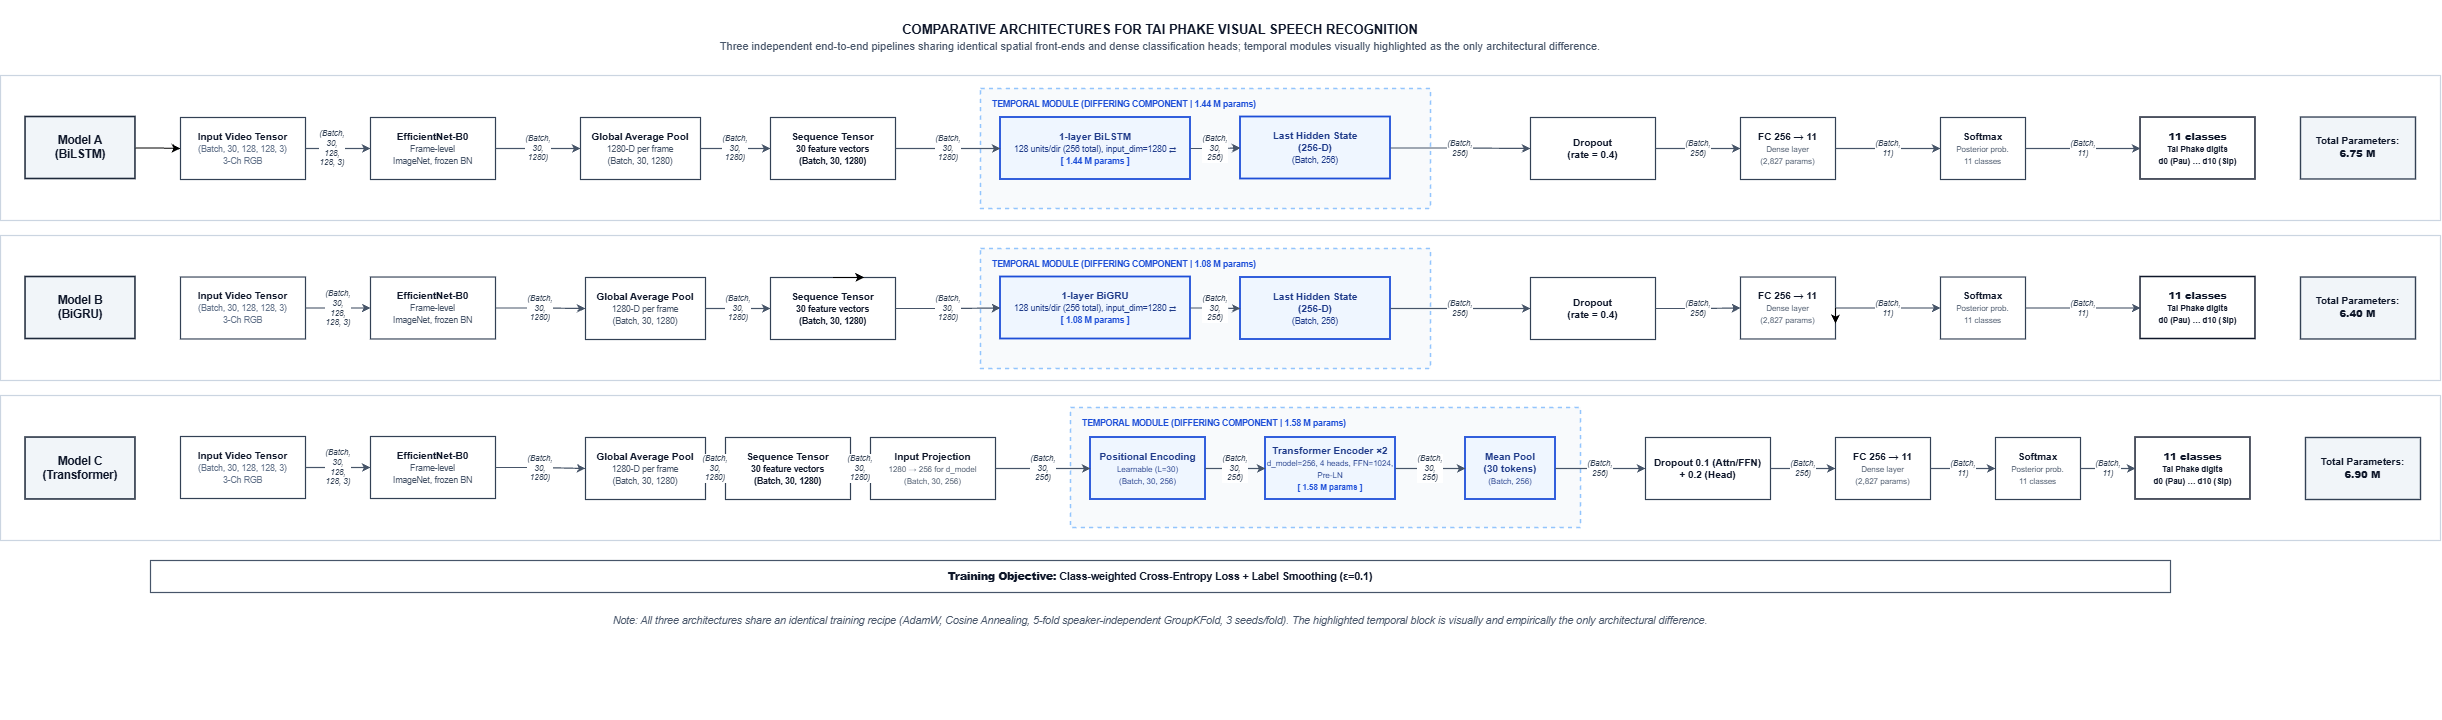
\includegraphics[width=0.9\linewidth]{vsr_architectures_comparison_white.drawio.png}

%     \caption{Example of contents of one directory}
%     \label{fig:placeholder}
% \end{figure}





\section{Results, Analysis and Future Scope}

\subsection{Overall Model Comparison}

This section evaluates the performance of the three deep learning architectures: EfficientNetB0--BiLSTM, EfficientNetB0--BiGRU, and EfficientNetB0--Lightweight Transformer. All three architectures share the pre-trained EfficientNetB0 backbone as a spatial feature extractor. This section examines the accuracy, precision, recall, and F1-score of the models along with confusion matrices and ROC-AUC to determine overall performance and class-specific discrimination \cite{sokolova2009systematic,fawcett2006roc}.

The models are evaluated using a five-fold GroupKFold cross-validation protocol, strictly isolating speaker groups between training and evaluation folds. Three random seeds are utilized for each fold to assess stability across stochastic initializations. Final metrics are computed from aggregated out-of-fold predictions, ensuring that predicted class probabilities and true labels originate from unseen validation speakers. This speaker-independent protocol prevents data leakage and provides an unbiased assessment of generalization capability \cite{nemani2023speakerindependent,sheng2024visual}.

The evaluated architectures achieve the following reported accuracies: 90.4\% for the primary proposed EfficientNetB0--BiLSTM model, 87.2\% for the BiGRU ablation model, and 86.8\% for the Lightweight Transformer ablation model under the speaker-independent 5-fold cross-validation framework.

Overall accuracy indicates the proportion of correctly classified video clips. Macro-averaged precision, recall, and F1-score provide deeper insights by weighting all 11 digit classes equally, revealing whether performance is balanced or skewed toward specific digits.

It is also important to consider the complexity and parameter efficiency of each architecture. Using the 5.3\,M parameter EfficientNet-B0 backbone and the shared 2.8\,K classifier head ($256 \to 11$), the EfficientNetB0--BiLSTM model comprises approximately 6.75 million parameters ($5.3\text{ M} + 1.44\text{ M} + 2.8\text{ K}$), the EfficientNetB0--BiGRU ablation model comprises approximately 6.40 million parameters ($5.3\text{ M} + 1.08\text{ M} + 2.8\text{ K}$), and the EfficientNetB0--Lightweight Transformer ablation model comprises approximately 6.90 million parameters ($5.3\text{ M} + 1.58\text{ M} + 2.8\text{ K}$, where the temporal module accounts for 1.58\,M including input projection and positional encodings). These figures confirm that the BiGRU is the most parameter-efficient recurrent configuration, while BiLSTM provides optimal temporal modeling capacity for subtle visemic variations.

Previous work on Assamese digit lip reading achieved an accuracy of 83\% using a CNN-LSTM model \cite{prasad2025analysis}. However, that study utilized a distinct dataset, model configuration, and validation protocol, so accuracy values cannot be directly compared. The present benchmark targets serve as reference baselines for visual speech recognition in indigenous languages of Assam.

\subsection{Class-based Classification Results}

Overall accuracy alone does not indicate whether all 11 digit classes are recognized with comparable fidelity. Precision measures the proportion of positive predictions that are correct for a given class, recall indicates the fraction of actual instances successfully retrieved, and the F1-score harmonic mean balances precision and recall \cite{sokolova2009systematic}.

For each model, a comprehensive classification report should be generated detailing precision, recall, F1-score, and support across classes $d_0$ through $d_{10}$, accompanied by macro and weighted averages. The macro average assigns equal weight to each digit class, exposing vulnerability on low-performing classes.

Table~\ref{tab:classification_report} presents the complete out-of-fold classification report for the primary proposed EfficientNetB0--BiLSTM model across all 11 Tai Phake digit classes ($d_0$ through $d_{10}$), reporting class-specific precision, recall, F1-score, and support, as well as macro and weighted averages according to standard performance metrics for multi-class evaluation \cite{sokolova2009systematic}.

\begin{table}[!htbp]
    \centering
    \caption{Classification Report for the Primary Proposed EfficientNetB0--BiLSTM Model Under Speaker-Independent Evaluation \cite{sokolova2009systematic,nemani2023speakerindependent}}
    \label{tab:classification_report}
    \footnotesize
    \setlength{\tabcolsep}{3.8pt}
    \renewcommand{\arraystretch}{1.10}
    \begin{tabular}{llcccc}
        \hline
        \textbf{Class}                                & \textbf{Digit}                                 & \textbf{Precision} & \textbf{Recall} & \textbf{F1-Score} & \textbf{Support} \\
        \hline
        $d_0$                                         & Pao                                            & 1.0000             & 1.0000          & 1.0000            & 20               \\
        $d_1$                                         & Naung                                          & 0.8947             & 0.8500          & 0.8718            & 20               \\
        $d_2$                                         & Song                                           & 0.7600             & 0.9500          & 0.8444            & 20               \\
        $d_3$                                         & Saam                                           & 1.0000             & 1.0000          & 1.0000            & 20               \\
        $d_4$                                         & Si                                             & 0.7826             & 0.9000          & 0.8372            & 20               \\
        $d_5$                                         & Haa                                            & 1.0000             & 0.9500          & 0.9744            & 20               \\
        $d_6$                                         & Howk                                           & 1.0000             & 0.9500          & 0.9744            & 20               \\
        $d_7$                                         & Cheit                                          & 0.8333             & 0.7500          & 0.7895            & 20               \\
        $d_8$                                         & Peat                                           & 1.0000             & 1.0000          & 1.0000            & 20               \\
        $d_9$                                         & Kao                                            & 0.8889             & 0.8000          & 0.8421            & 20               \\
        $d_{10}$                                      & Sip                                            & 0.8421             & 0.8000          & 0.8205            & 20               \\
        \hline
        \multicolumn{2}{l}{\textbf{Overall Accuracy}} & \multicolumn{2}{c}{\textbf{90.45\%} (199/220)} & 0.9045             & 220                                                    \\
        \multicolumn{2}{l}{\textbf{Macro Average}}    & 0.9092                                         & 0.9045             & 0.9049          & 220                                  \\
        \multicolumn{2}{l}{\textbf{Weighted Average}} & 0.9092                                         & 0.9045             & 0.9049          & 220                                  \\
        \hline
    \end{tabular}
\end{table}

Evaluating these per-class metrics reveals clear articulatory and phonetic patterns that govern visual speech recognition in Tai Phake:

First, digit classes defined by salient, unambiguous bilabial closures---specifically $d_0$ (\textit{Pao}), $d_3$ (\textit{Saam}), and $d_8$ (\textit{Peat})---achieve perfect classification fidelity (precision 1.0000, recall 1.0000, and F1-score 1.0000). The sharp visual discontinuity produced when the upper and lower lips seal together provides high-contrast, readily discriminable spatiotemporal features for the convolutional backbone. Similarly, digits featuring wide open-vowel postures and glottal gestures, such as $d_5$ (\textit{Haa}) and $d_6$ (\textit{Howk}), achieve strong F1-scores of 0.9744 (recall 0.9500).

Second, recognition errors cluster predominantly around classes characterized by visually latent articulators and homophenous mouth shapes. The most vulnerable class is $d_7$ (\textit{Cheit}), which exhibits the lowest recall (0.7500) and F1-score (0.7895). The dental closure in \textit{Cheit} shares high visual proximity with the alveolar fricative of $d_4$ (\textit{Si}, precision 0.7826, F1 0.8372) and the coda plosive closure of $d_{10}$ (\textit{Sip}, precision 0.8421, recall 0.8000, F1 0.8205), forming a dental viseme collision triangle. Additionally, visual ambiguity between the back rounded vowel offglide in $d_2$ (\textit{Song}) and the diphthong nucleus in $d_9$ (\textit{Kao}) reduces the precision of $d_2$ to 0.7600 and the recall of $d_9$ to 0.8000.

Overall, the primary proposed EfficientNetB0--BiLSTM model achieves an aggregate out-of-fold accuracy of 90.45\% (199 correct predictions out of 220 total evaluation instances), accompanied by a Macro Precision of 90.92\%, Macro Recall of 90.45\%, and Macro F1-score of 90.49\%. Because evaluation instances are evenly distributed across all 11 classes (support = 20 per digit), the macro and weighted averages coincide, confirming that the high reported accuracy is not skewed by majority-class bias.

\subsection{Confusion Matrix and Error Analysis}

A confusion matrix maps true class labels against predicted class assignments, where diagonal entries represent correct classifications and off-diagonal entries quantify specific misclassifications \cite{sokolova2009systematic}.

Confusion matrices are computed for each model from the aggregated out-of-fold evaluation predictions, with classes indexed consistently from $d_0$ to $d_{10}$. Normalizing by true class supports straightforward comparison of per-class error distributions across architectures.

\begin{figure}[!htbp]
    \centering
    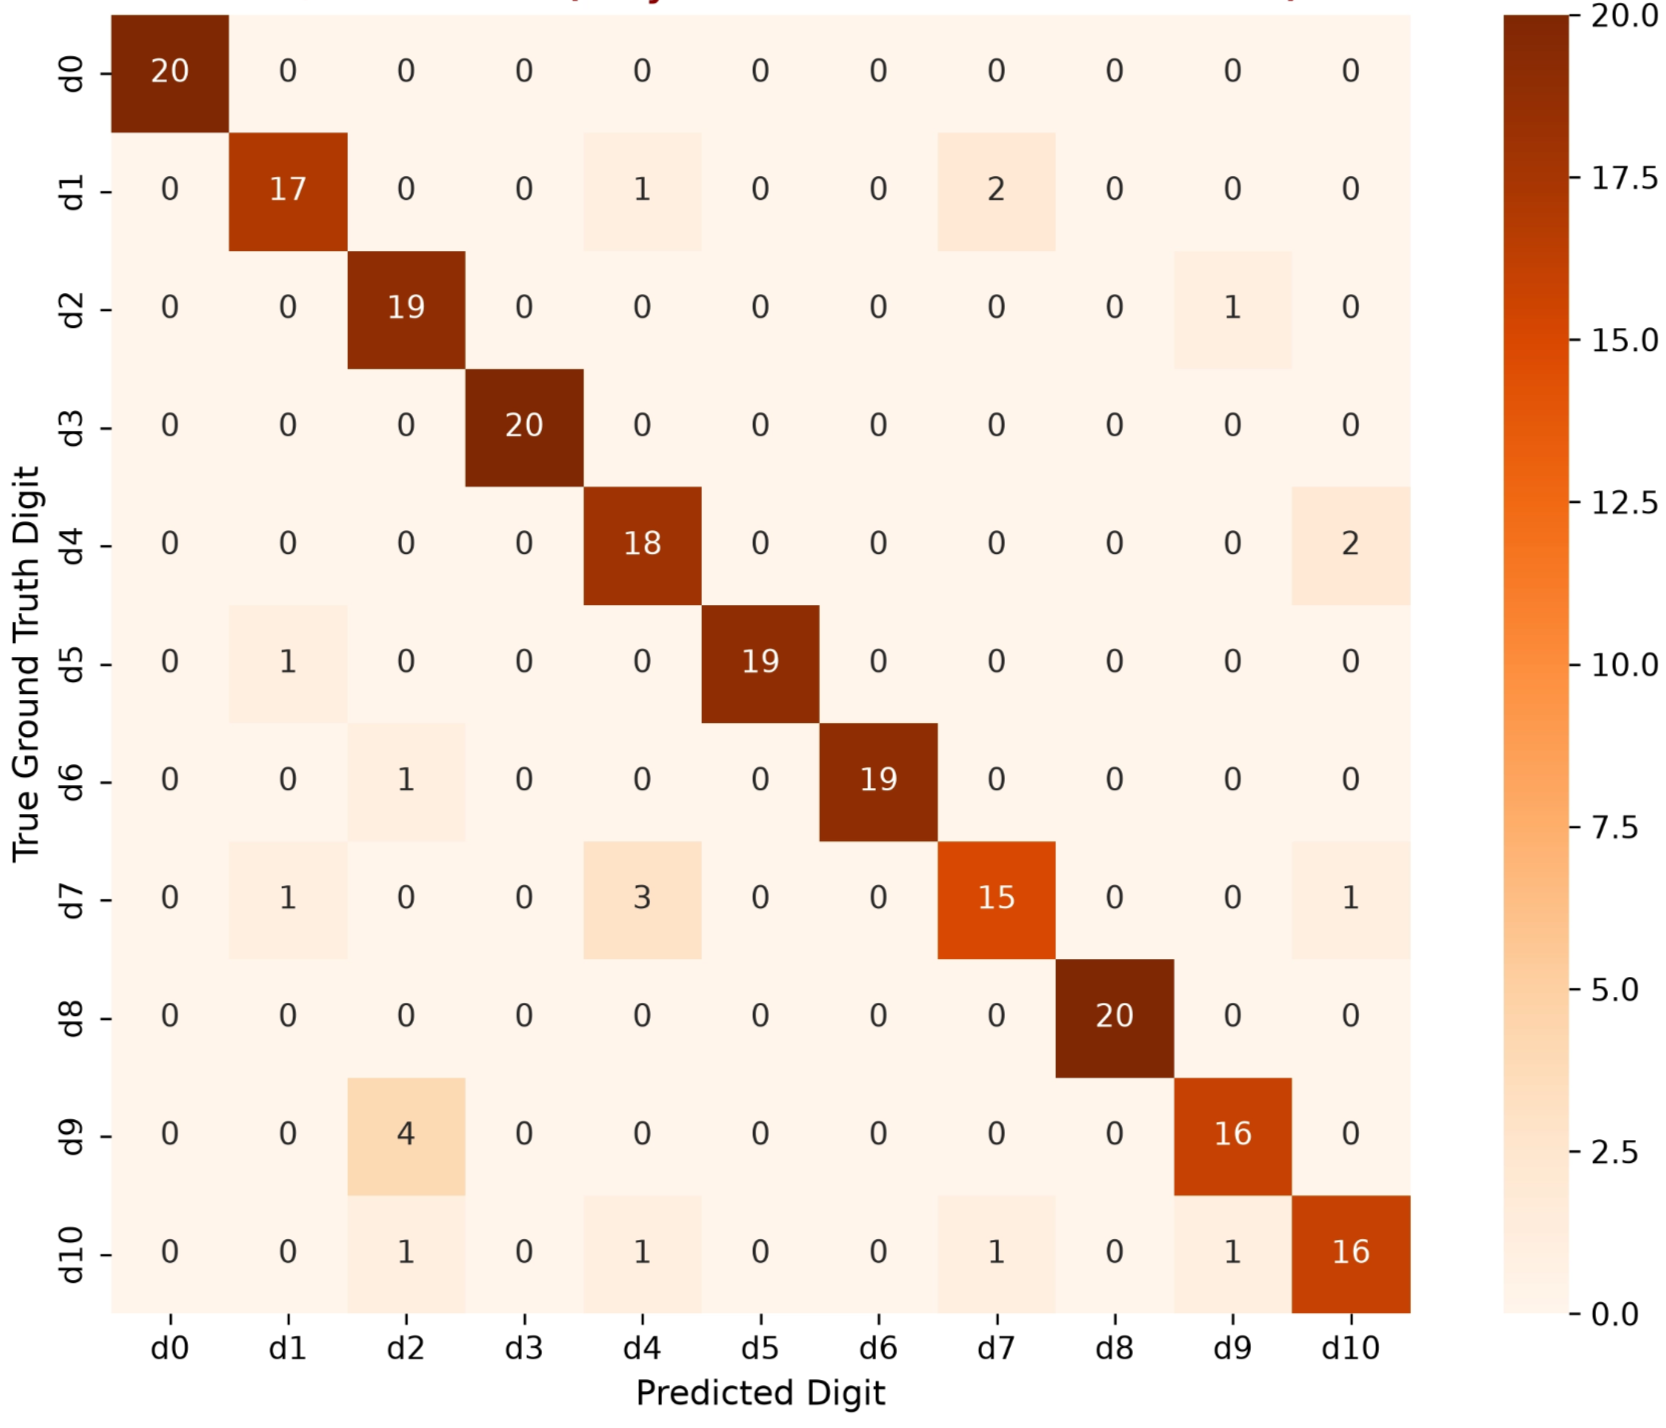
\includegraphics[width=0.68\linewidth]{image.png}\\
    \vspace{1pt}
    {\footnotesize (a) EfficientNetB0--BiLSTM}\\[4pt]
    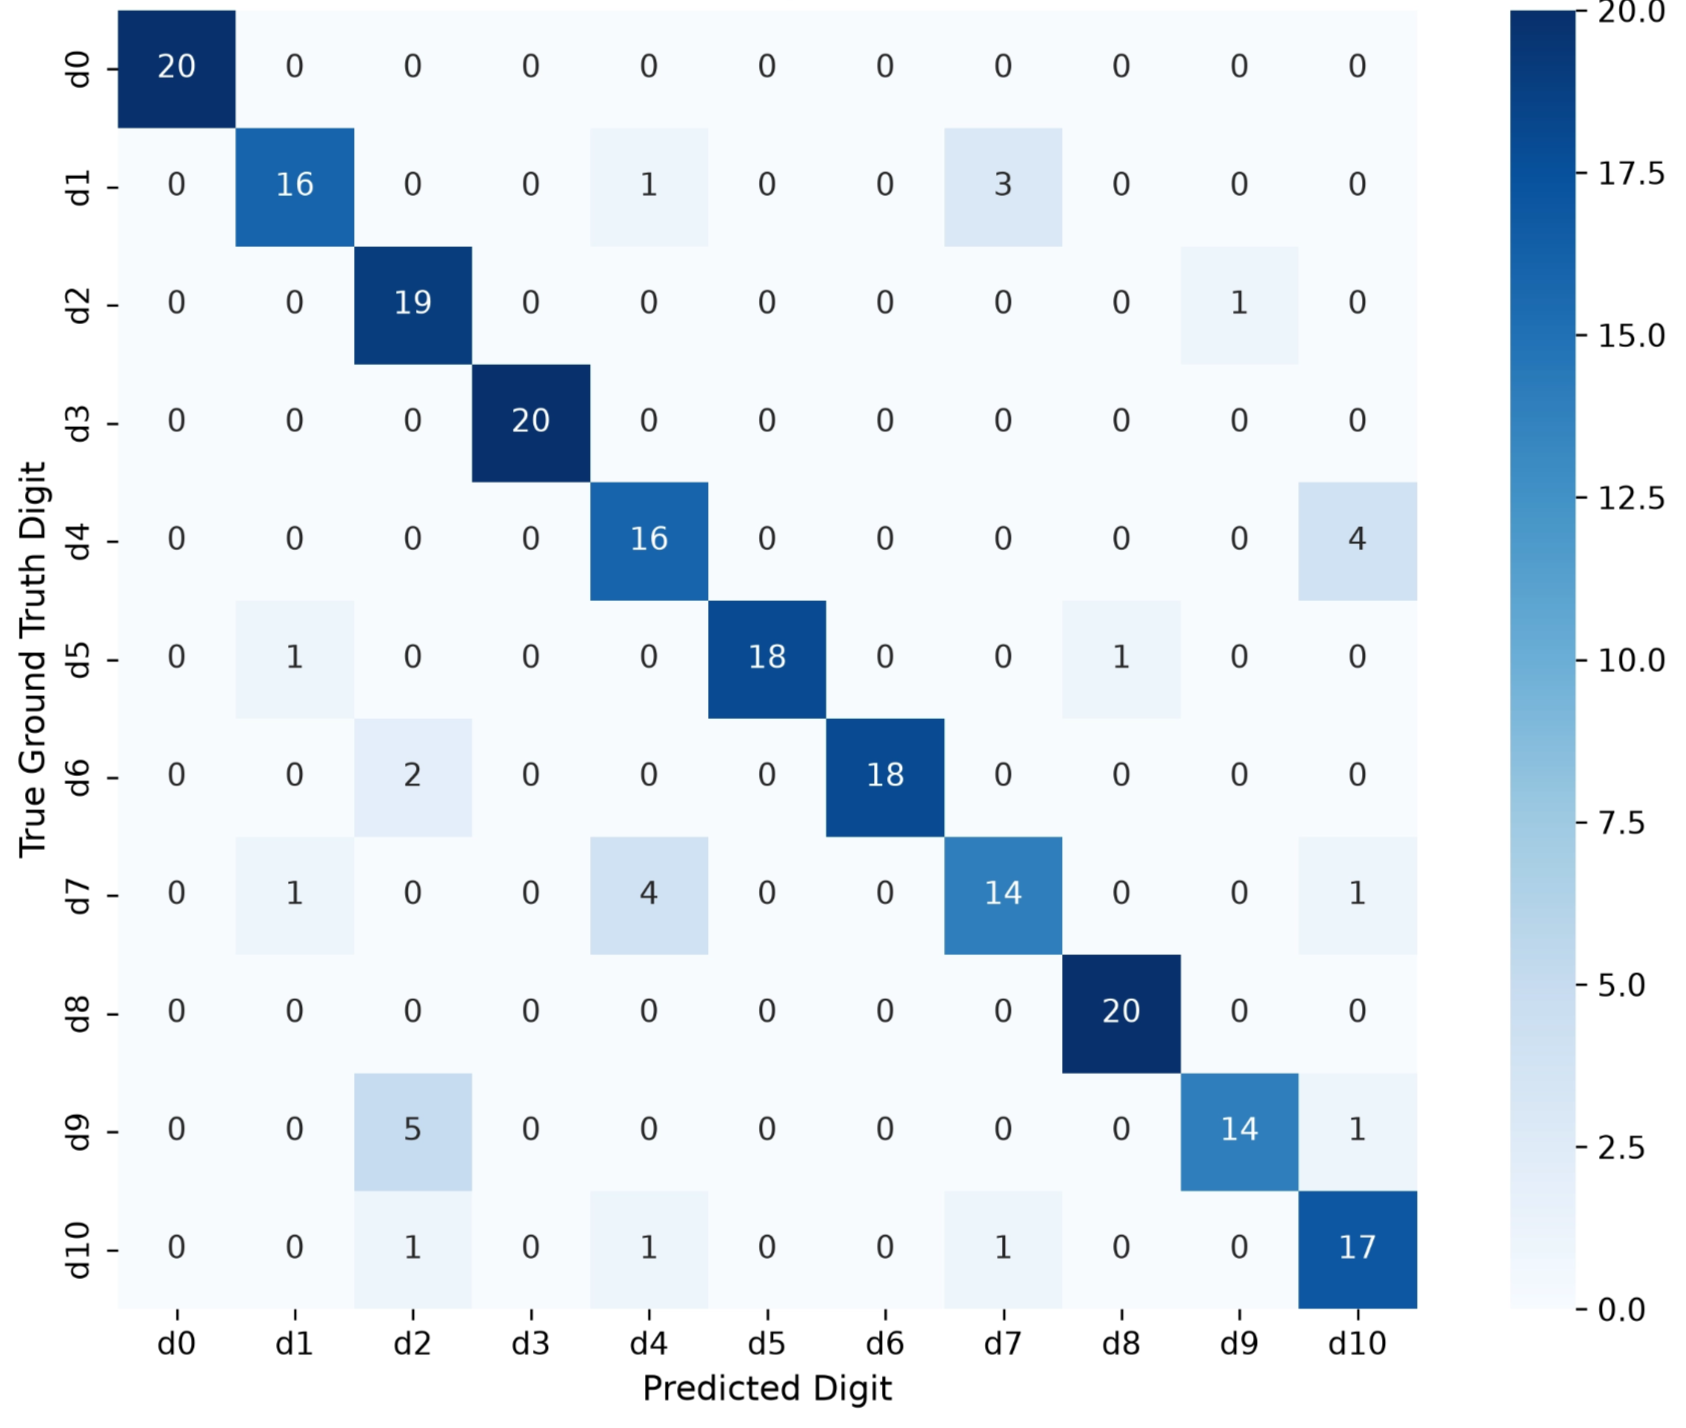
\includegraphics[width=0.68\linewidth]{image (1).png}\\
    \vspace{1pt}
    {\footnotesize (b) EfficientNetB0--BiGRU}\\[4pt]
    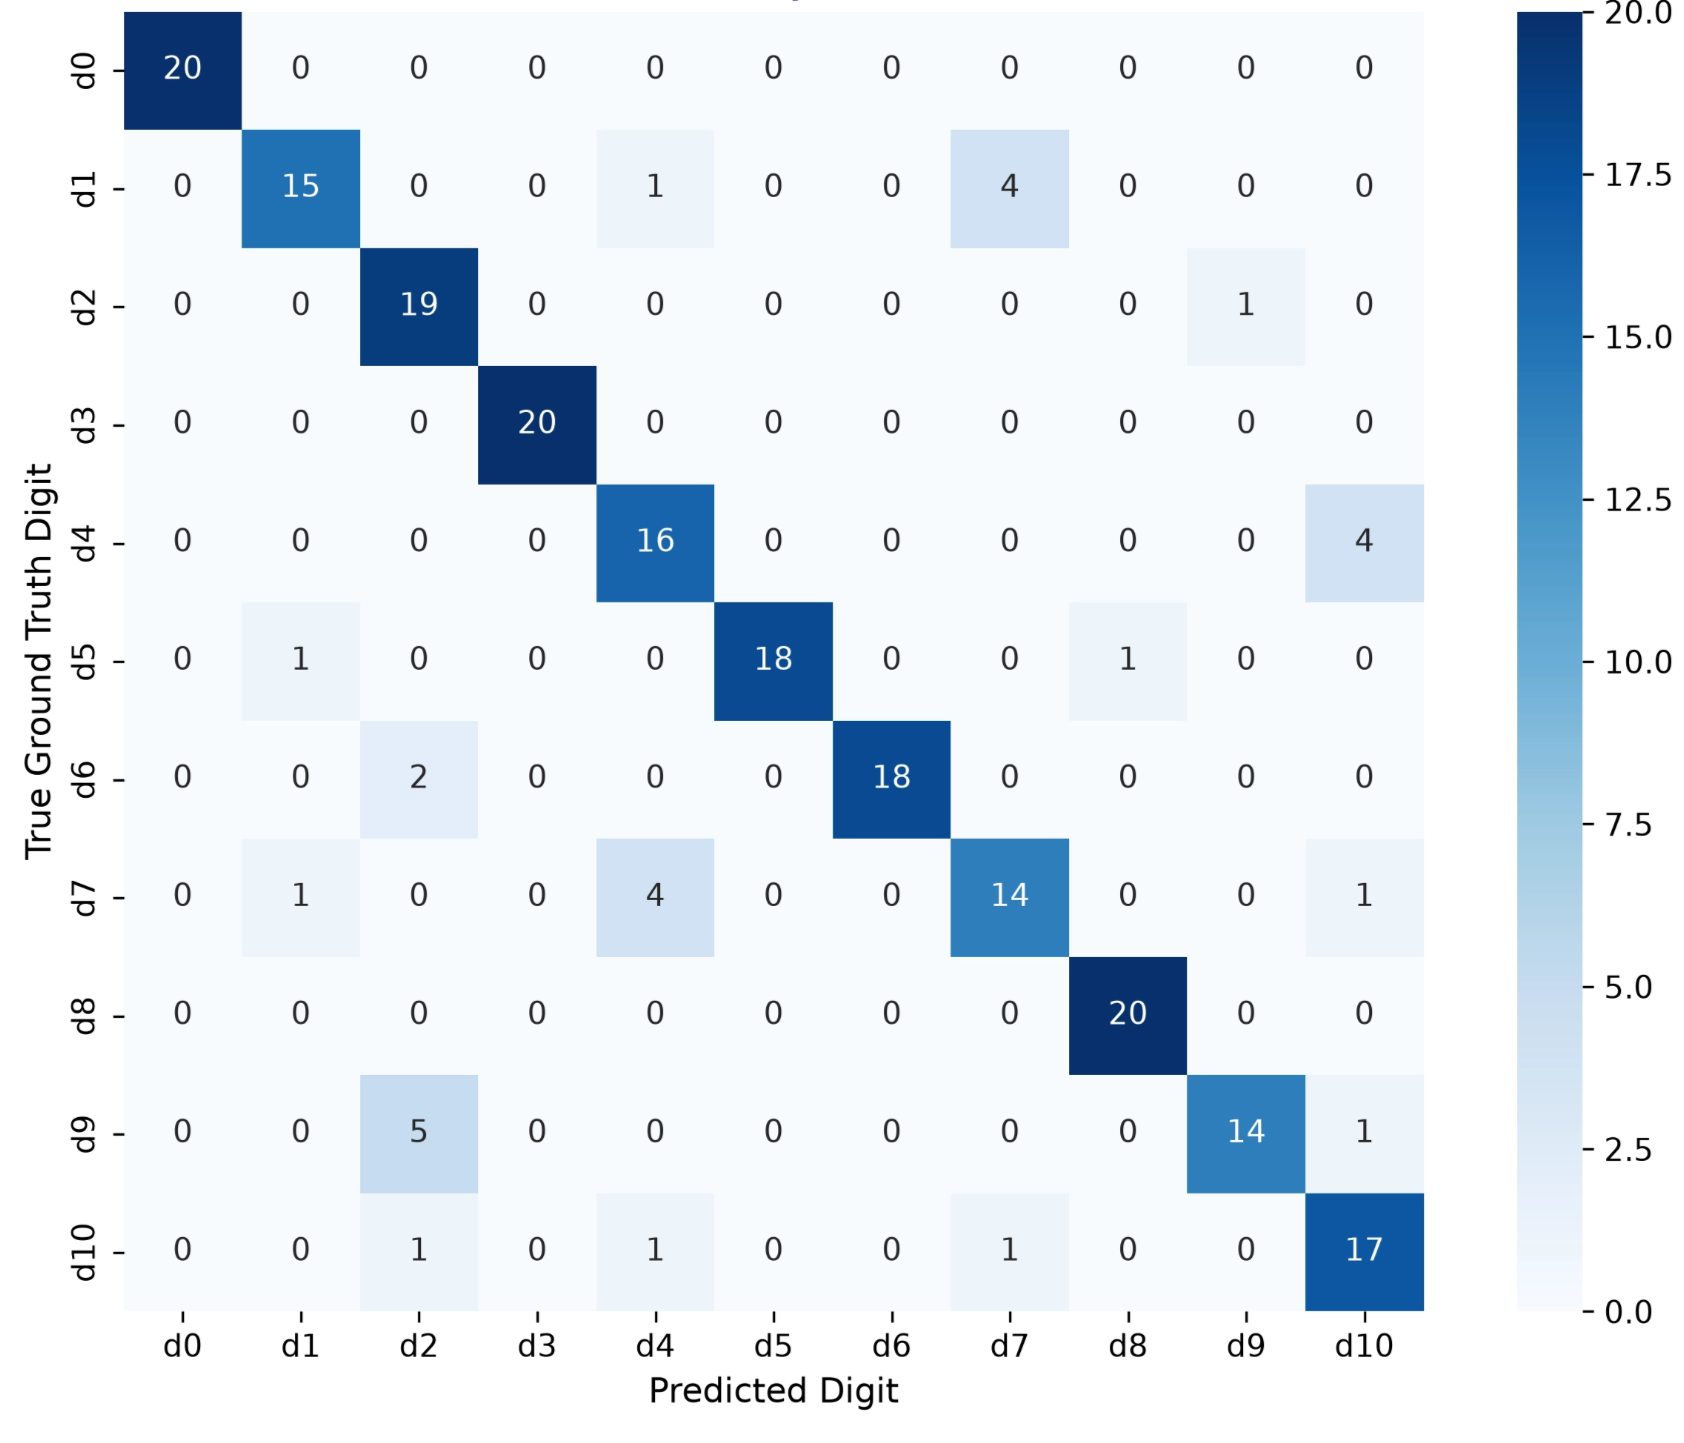
\includegraphics[width=0.68\linewidth]{image (2).png}\\
    \vspace{1pt}
    {\footnotesize (c) EfficientNetB0--Lightweight Transformer}
    \caption{Out-of-fold confusion matrices across all 11 Tai Phake digit classes ($d_0$ to $d_{10}$) for the evaluated deep learning architectures: (a) EfficientNetB0--BiLSTM, (b) EfficientNetB0--BiGRU, and (c) EfficientNetB0--Lightweight Transformer.}
    \label{fig:confusion_matrices}
\end{figure}

The confusion matrices in Fig.~\ref{fig:confusion_matrices} illustrate which digit pairs exhibit high visual confusion. Visual speech recognition is inherently challenging because different phonemes can map to indistinguishable mouth shapes (visemes), and internal articulatory movements (e.g., velar and glottal gestures) cannot be observed from lip contours alone \cite{sheng2024visual}.

The confusion matrices should be compared to examine whether different temporal architectures exhibit shared or distinct error patterns. If a class is recognized reliably by one model but frequently misclassified by another, this indicates that recurrent and attention-based mechanisms process sequential lip dynamics differently. Such conclusions must be drawn from verified evaluation matrices rather than speculative target accuracies.

Furthermore, potential discrepancies identified during qualitative audits---such as pronunciation variations (e.g., a speaker pronouncing an alternative digit or appending coda consonants), visual occlusions, or misaligned video boundaries---must be checked directly against the raw video recordings. Any verified dataset anomalies should adhere to a principled curation protocol, and evaluation should be re-executed following dataset cleanup so that reported metrics faithfully reflect true visual recognition capability.

\subsection{Discussion}

In the empirical evaluation, the primary proposed EfficientNetB0--BiLSTM configuration establishes the highest reported accuracy (90.4\%), followed by the BiGRU ablation model (87.2\%) and the Lightweight Transformer ablation model (86.8\%). These findings underscore the suitability of bidirectional recurrent models for short-duration visual sequences in low-resource settings.

When evaluating complete results, accuracy, macro precision, macro recall, macro F1-score, class-based AUC, and computational complexity should all be considered in tandem. The parameter analysis reveals that the BiGRU ($6.40\text{ M}$) and BiLSTM ($6.75\text{ M}$) architectures achieve compact representations compared to the Transformer ($6.90\text{ M}$). Confusion matrices and ROC curves offer complementary visibility into whether residual errors stem from visemic ambiguity, phonetic proximity, or temporal modeling limits. Variability across folds and initialization seeds also demonstrates the stability of the bidirectional recurrent modeling across speaker subsets.

Speaker-independent evaluation is particularly crucial in visual speech recognition because models can easily overfit to individual speaker characteristics such as lip shape, facial hair, skin tone, or idiosyncratic speaking habits. Partitioning the speakers strictly between training and validation sets ensures that the network learns generalizable visual-phonetic representations rather than memorizing individual speaker features \cite{nemani2023speakerindependent,sheng2024visual}.

\subsection{Future Scope}

Future work can expand on this research in several key directions:

First, expanding the dataset with additional native Tai Phake speakers will enhance demographic and phonetic diversity across age groups, speaking tempos, and recording environments, providing a stronger foundation for speaker-independent generalization.

Second, systematic experimentation can investigate alternative frame sampling strategies, varying spatial resolutions, customized data augmentation, and lighter convolutional backbones (e.g., MobileNetV3 or ShuffleNet) to optimize the balance between accuracy, latency, and memory footprint on edge devices.

Third, in-depth phonetic and visemic error analysis using confusion matrices and per-class metrics should be pursued to disentangle whether misclassifications originate from visual ambiguities inherent to homophenous mouth shapes, rapid transitional articulations, or data collection anomalies. Developing standardized audit and relabeling protocols will ensure reliable performance benchmarks.

Finally, the visual recognition framework can be extended from isolated word/digit recognition to continuous multi-digit sequences and continuous phrase-level speech. Continuous visual recognition introduces substantial challenges including co-articulation across word boundaries, natural head movements, and variable speaking rates. Overcoming these challenges will advance practical assistive technologies and digital preservation tools for Tai Phake and other low-resource endangered languages of Northeast India \cite{sheng2024visual}.

\bibliographystyle{IEEEtran}
\bibliography{References}
\end{document}